\chapter{Experiments and Data Collection}\label{chapter:expt-data-collection}
In this section, we describe how the sleep experiments are conducted and fly video recordings data were collected.

\textit{The experimental data were collected by Dr. Mehmet Fatih Keles at Wu Lab, Johns Hopkins University.}

\section{Sleep Experiments and Video Recordings}
A custom imaging setup was used to perform high-resolution characterization of sleep-related behaviors in flies. This set up includes a custom 3D printed chamber (7.2X4.3X2.4 mm [WxHxL]) that is placed in front of an IR sensitive (Flir) 30 FPS camera with telecentric lens (Edmund Optics), an illustration of the experiment setup is given in the Figure~\ref{figure:experiment-setup}.

\begin{table}[htb!]
	\begin{adjustbox}{width=1\textwidth}
		\begin{tabular}{c c c c}
			\toprule
			\multicolumn{1}{c}{\textbf{Experiment Name}} & \multicolumn{1}{c}{\textbf{Experiment Type}} & \multicolumn{1}{c}{\textbf{Fly Gender}} & \multicolumn{1}{c}{\textbf{\# of Frames}} \\
			\cmidrule(lr){1-1}\cmidrule(lr){2-2}\cmidrule(lr){3-3}\cmidrule(lr){4-4}
			FlyF1-03082020164520                         & wild type sleep                              & female                                  & 1727979                                   \\
			FlyF11-01182022175505                        & wild type sleep                              & female                                  & 1727979                                   \\
			FlyF14-08172021175459                        & wild type sleep                              & female                                  & 1727979                                   \\
			FlyF15-08182021173222                        & wild type sleep                              & female                                  & 1727979                                   \\
			FlyF8-08112021174107                         & wild type sleep                              & female                                  & 1727979                                   \\
			FlyM13-08172021175457                        & wild type sleep                              & male                                    & 1727979                                   \\
			FlyM4-03062020153616                         & wild type sleep                              & male                                    & 1727979                                   \\
			FlyF19SD-11052021164243                      & sleep deprived                               & female                                  & 2159979                                   \\
			FlyF19SD-11152020170647                      & sleep deprived                               & female                                  & 2159979                                   \\
			FlyF41SD-11192021170807                      & sleep deprived                               & female                                  & 2159979                                   \\
			FlyF52SD-11242021161943                      & sleep deprived                               & female                                  & 2159979                                   \\
			\bottomrule
		\end{tabular}
	\end{adjustbox}
	\caption{Collected experiment data details. \label{table:experiment-details}}
\end{table}

\begin{figure}[htb!]
	\centering
	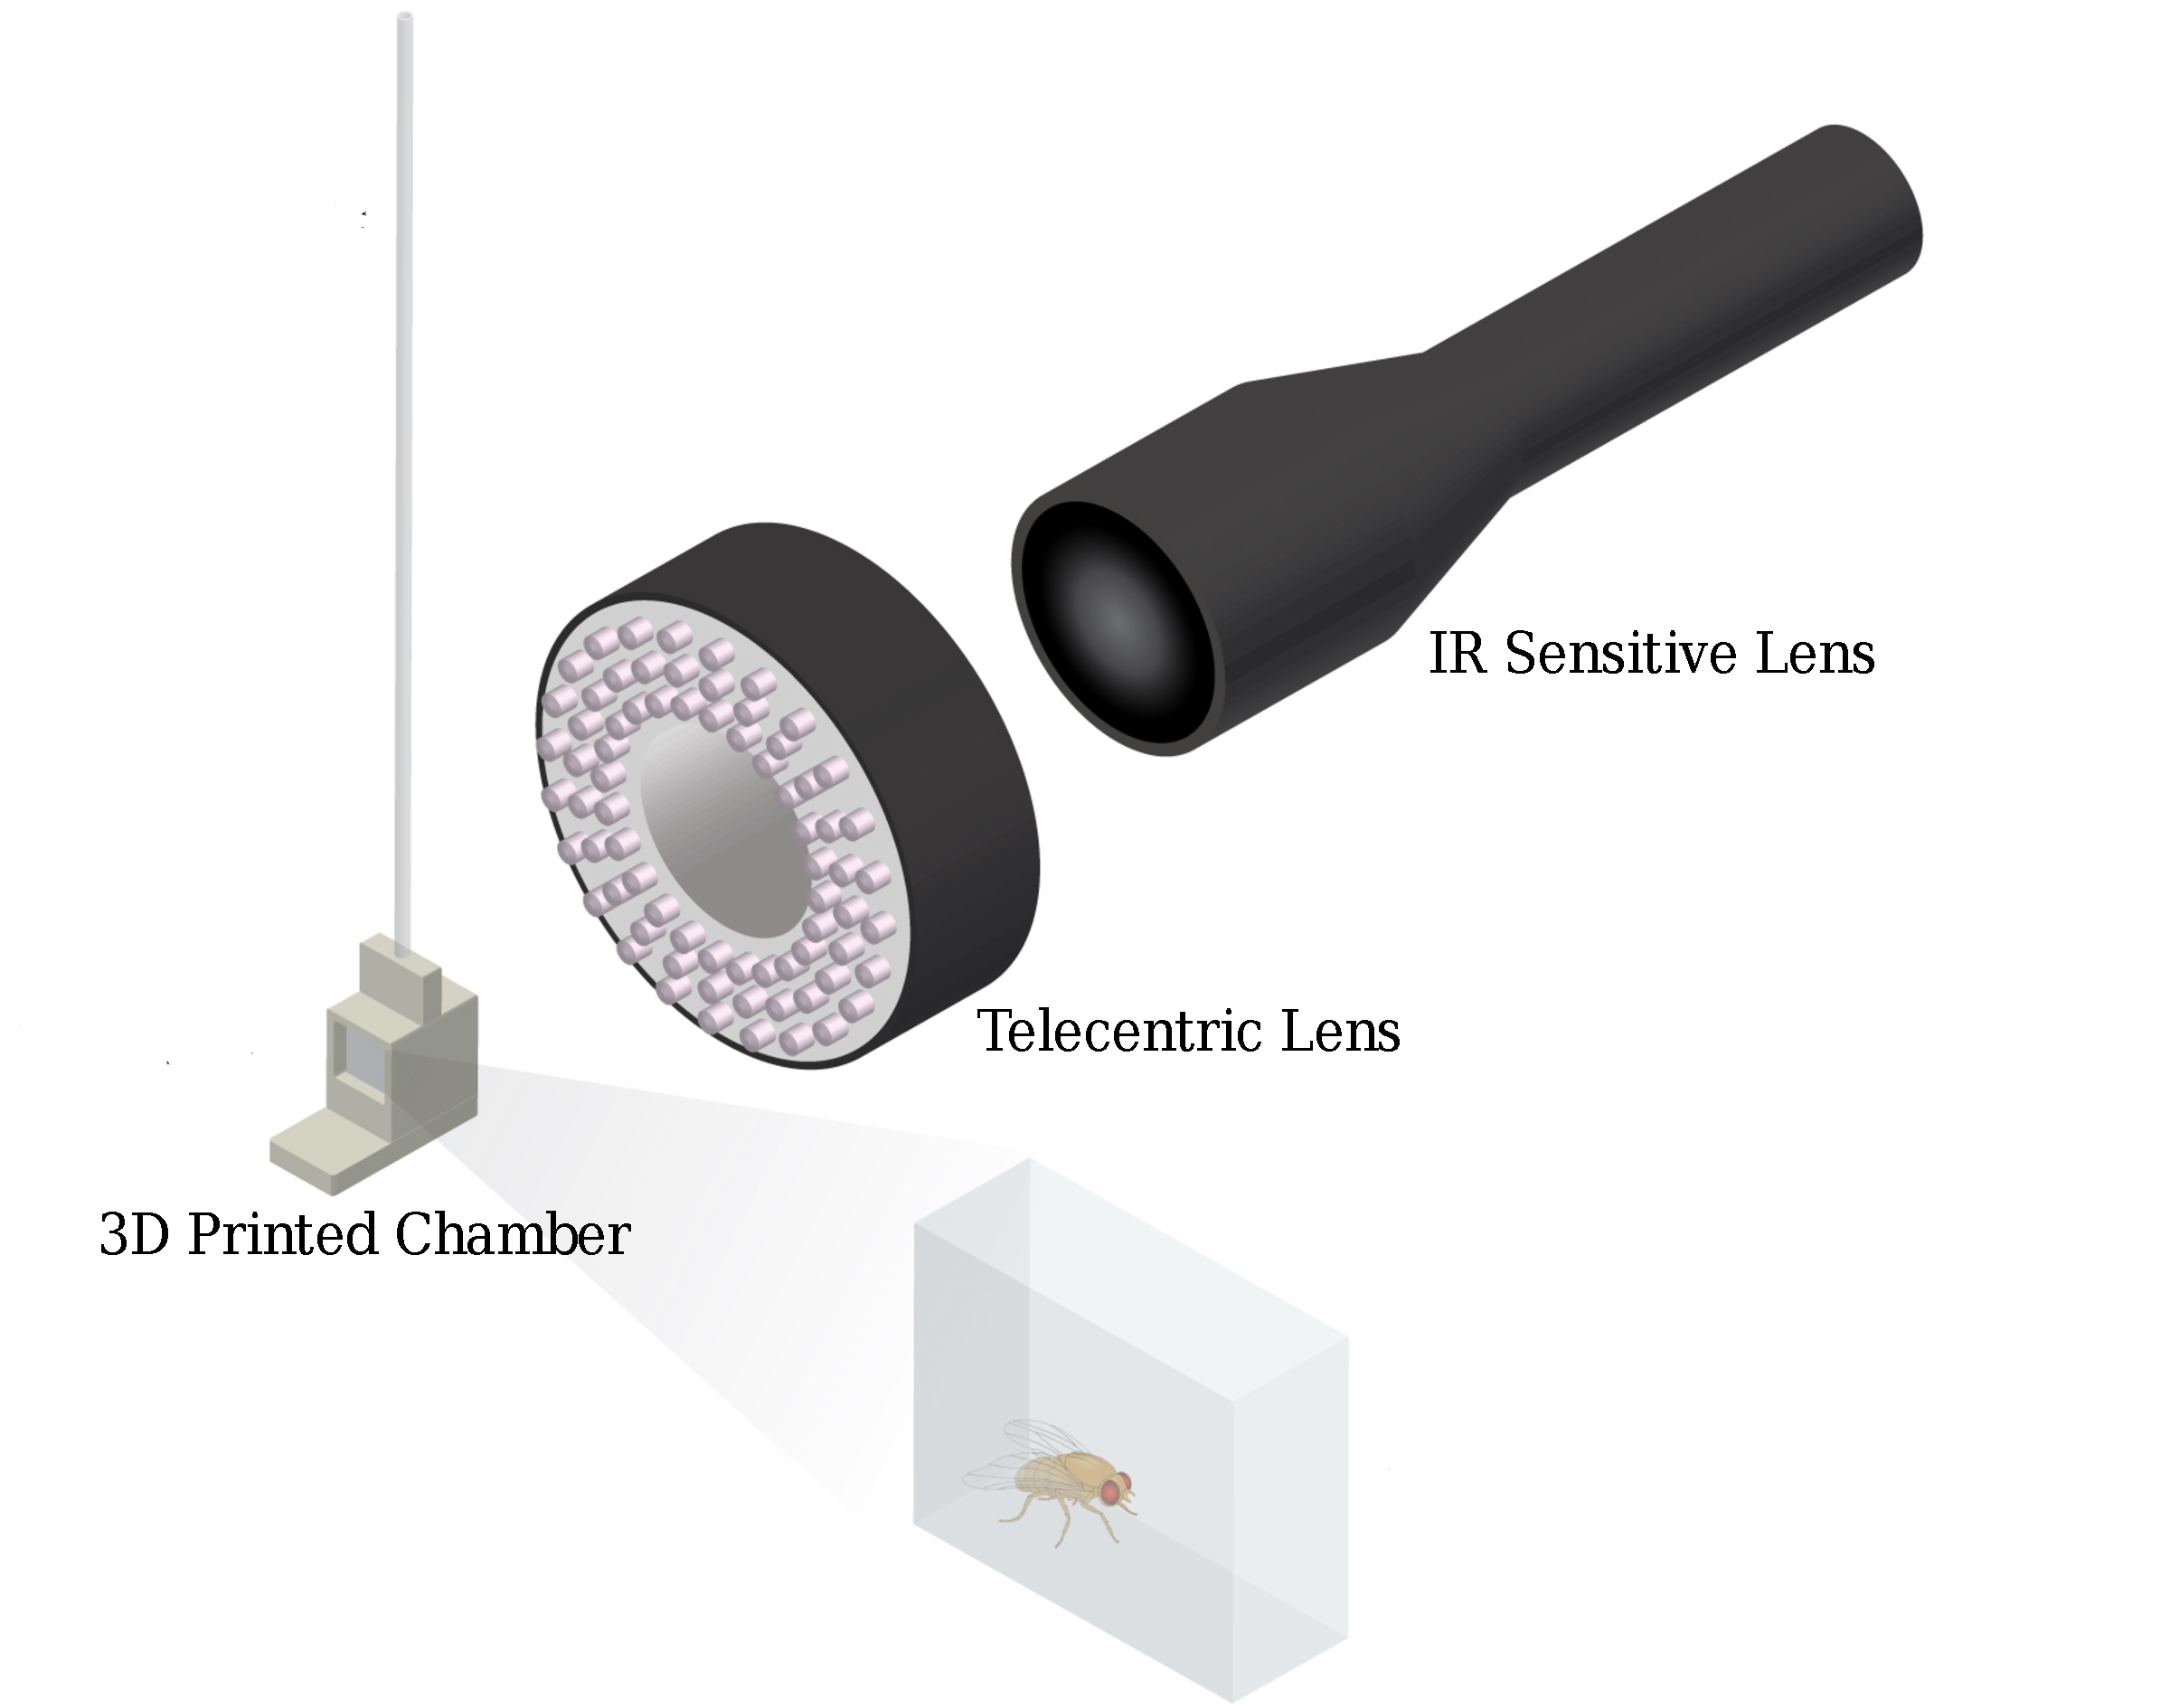
\includegraphics[width=0.8\linewidth]{figures/ExperimentalSetup.pdf}
	\caption[An illustration of the experimental setup which is used to perform high-resolution imaging of experiments.]{An illustration of the experimental setup which is used to perform high-resolution imaging of experiments.\label{figure:experiment-setup}}
\end{figure}

Flies recorded between ZT10-ZT2 (16 hours total) for wild type sleep experiments, and between ZT10-ZT6 (20 hours total) for sleep-deprived experiments (see Table~\ref{table:experiment-details}).
Each chamber has a food port (1.5 mm diameter) that allows access to liquid food (2.5\% yeast, 2.5\% sugar).
Recording setup is in a light tight box and humidity control (60\%) is achieved via a humidifier plugged into a humidity control switch. Experimental flies are loaded to individual chambers at ZT8-ZT9 via mouth pipette or a small vacuum pump.
Individual chambers are sealed with a 7×7 mm acrylic windows.
Windows are coated with SigmaCote to prevent flies from ventral or dorsal postural positions. 5-7 day old female and male flies are used in the experiments.

\section{Pose Estimation and Tracking}
A recently developed deep neural network based software, DeepLabCut \citep{mathis_deeplabcut_2018} was used to achieve markerless pose estimation.
Over 20 body parts are first labeled in 1654 images from 28 animals (16 female, 12 male) to train the model with a 95/5 train/test split. An example labeled frame is given in the Figure~\ref{figure:example-labeled-frame}.
We used a ResNet-50 \citep{he_deep_2016} based neural network with a batch size of 4 and 200,000 training iterations.
Rest of the settings were kept default.
The resulting network has a test error of 3.67 pixels.

\begin{figure}[htb!]
	\centering
	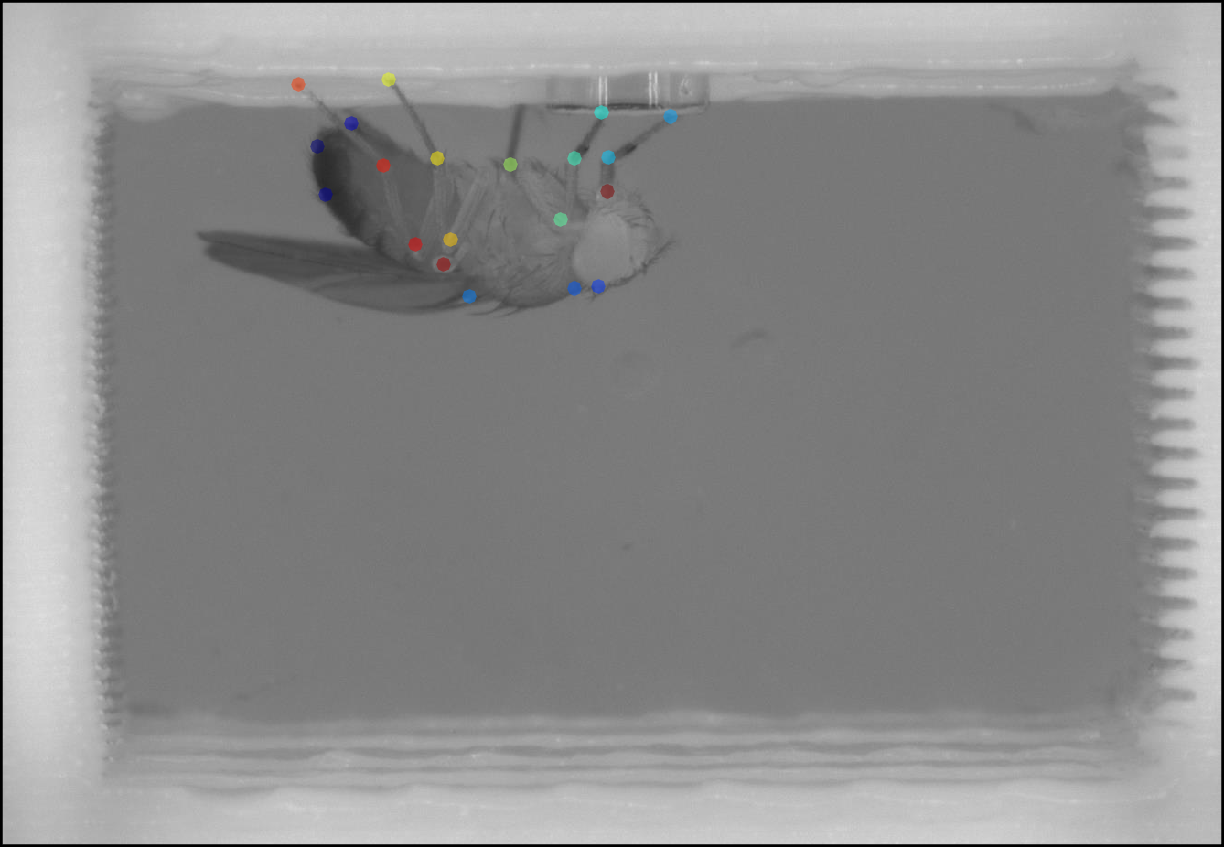
\includegraphics[width=0.6\linewidth]{figures/FlyTrackedBodyParts.png}
	\caption[An example frame of the fruit fly placed in 3D printed chamber.] {An example video recording frame of the fruit fly placed in 3D printed chamber. Colorful markers indicate the tracked body parts.\label{figure:example-labeled-frame}}
\end{figure}

\section{Behavior Annotations}
3 human annotators labeled 5 different behaviors (feeding, grooming, moving, haltere switch, proboscis pumping) across 11 videos (14 hours and 16 hours each, respectively for 7 wild type sleep experiments and 4 sleep deprivation experiments).
A single experiment is annotated by all 3 annotators to check rigor and overlap among annotators. We only used the annotations of a fly when each pair of annotators agreed at least on the 90\% of the annotations. Two example ethograms generated from the annotations are given in the Figure~\ref{figure:example-ethograms}.

\begin{figure}[b!]
	\centering
	\begin{subfigure}[ht!]{0.9\linewidth}
		\centering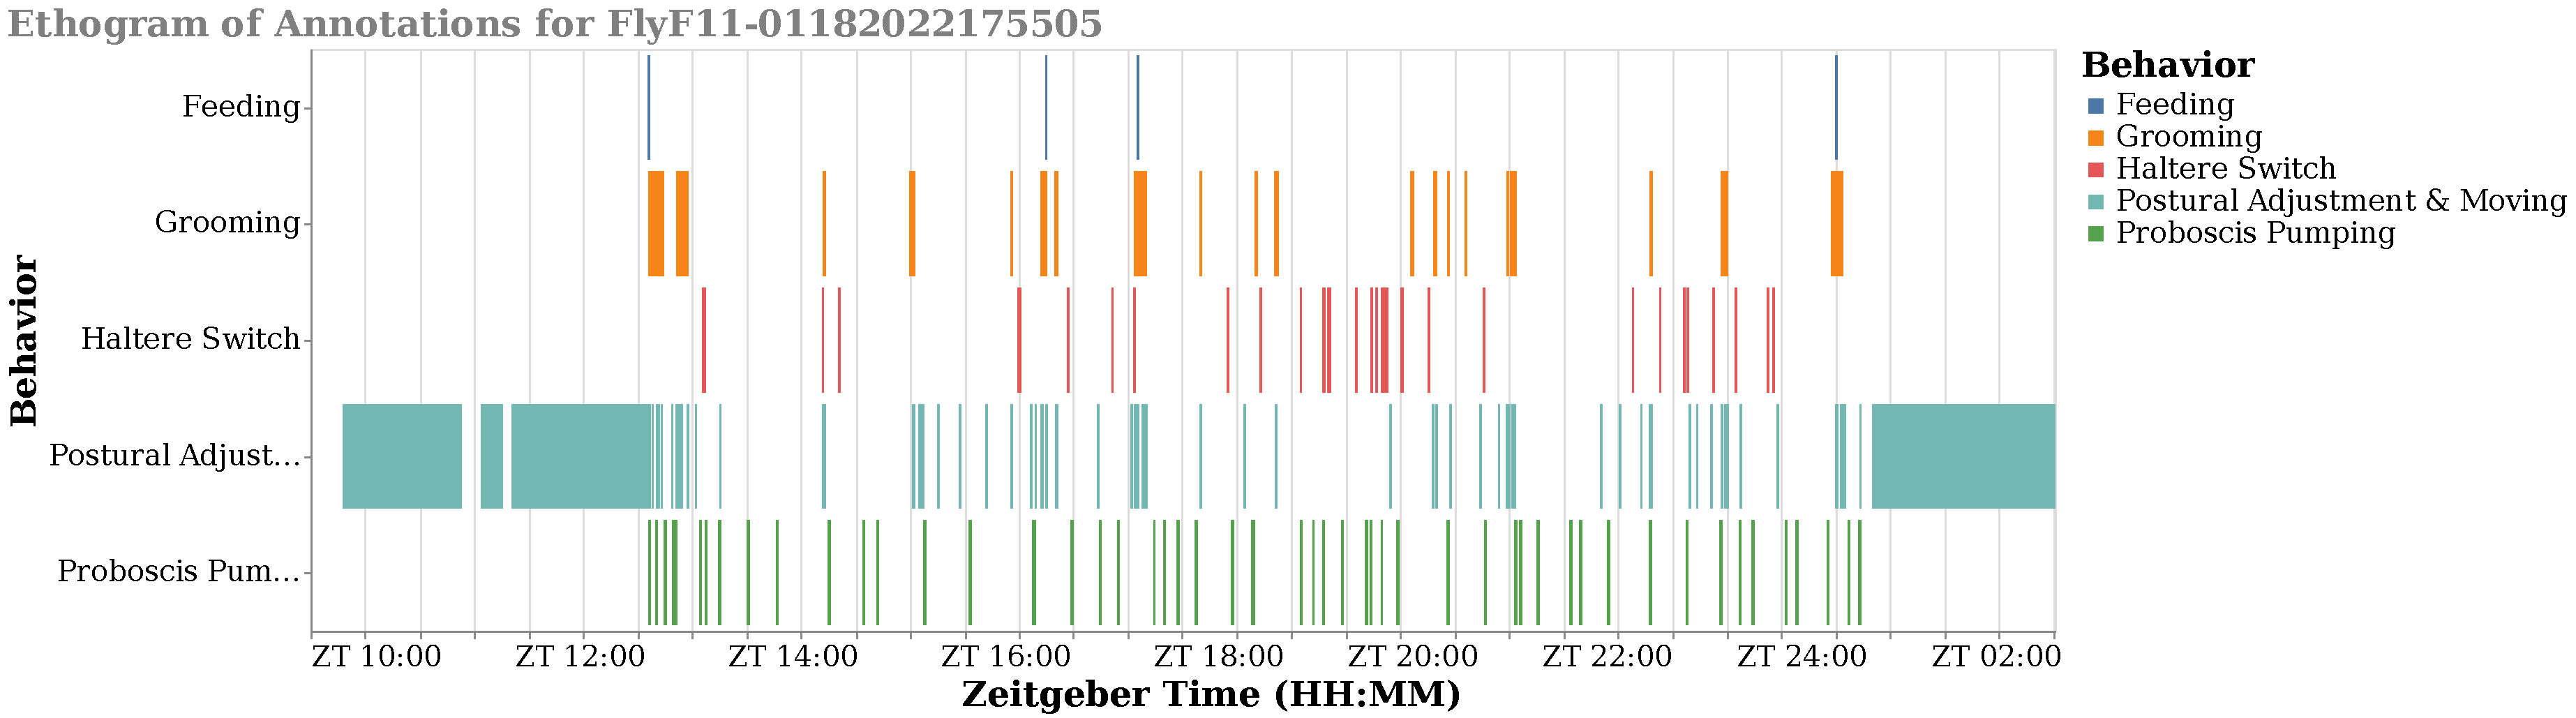
\includegraphics[width=\linewidth]{figures/FlyF11-01182022175505_annotation_ethogram.pdf}
		\caption{Wild type.}
	\end{subfigure}%

	\centering
	\begin{subfigure}[ht!]{0.9\linewidth}
		\centering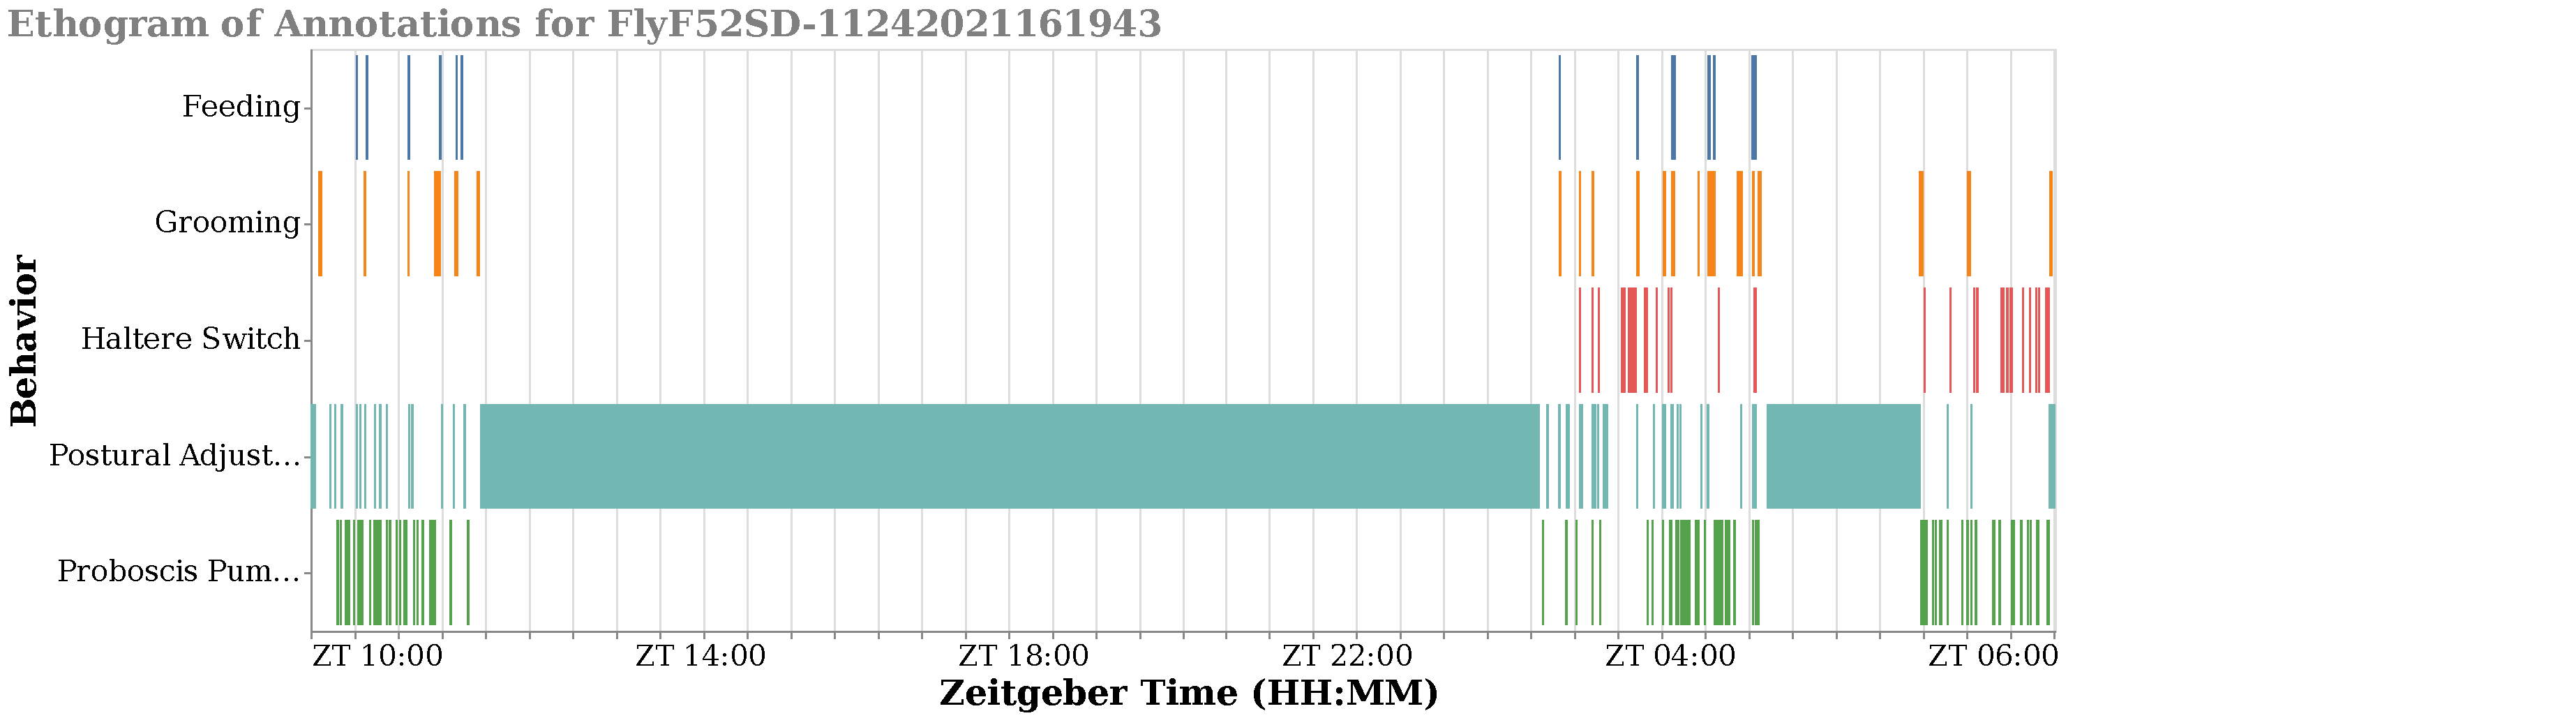
\includegraphics[width=\linewidth]{figures/FlyF52SD-11242021161943_annotation_ethogram.pdf}
		\caption{Sleep-deprived.}
	\end{subfigure}%
	\caption[Two example ethograms of annotated behaviors observed during the sleep experiments.]{Two example ethograms of annotated behaviors observed during the sleep experiments. Dark period starts at ZT12, and ends at ZT0. \label{figure:example-ethograms}}
\end{figure}
